\documentclass[10pt]{beamer}
\usepackage[utf8]{inputenc}
\usepackage[english]{babel}
\usepackage{alphabeta}
\usepackage{amsmath,amsthm,amsfonts,amssymb}
\usepackage{latexsym}
\usepackage[all,cmtip]{xy}
\usepackage{mathtools}
\usepackage{braket}
\usepackage[font=scriptsize,labelfont=bf]{caption}
\usepackage{tikz}
\usepackage{xmpmulti}
\usepackage{soul}

% set colors
\definecolor{myNewColorA}{RGB}{0, 109, 174}
\definecolor{myNewColorB}{RGB}{111, 100, 169}
\definecolor{myNewColorC}{RGB}{0, 111, 41}
\definecolor{myNewColorD}{RGB}{245, 123, 66}

\setbeamercolor*{titlelike}{fg=myNewColorA}
\setbeamercolor*{title}{bg=myNewColorA, fg = white}
\setbeamercolor*{caption name}{fg=myNewColorA}


% references
\usepackage{hyperref}

\newcommand*{\Scale}[2][4]{\scalebox{#1}{\ensuremath{#2}}}%
%------------------------------------------------------------

\setbeamerfont{title}{size=\large}
\setbeamerfont{subtitle}{size=\small}
\setbeamerfont{author}{size=\small}
\setbeamerfont{date}{size=\footnotesize}

\title{Faster than Hermitian Quantum Mechanics}
\subtitle{by Carl M Bender et al}
\author{Ana Fabela Hinojosa}
\institute[]{
\includegraphics[scale=0.18]{logo.jpg}}
\date[\today]{Supervisors:\\ Jesper Levinsen\\ Meera Parish } 
%------------------------------------------------------------
% This block of commands puts the table of contents at the 
% beginning of each section and highlights the current section:
\AtBeginSection[]
{
 \begin{frame}
    \frametitle{Contents}
    \tableofcontents[currentsection]
 \end{frame}
}

% ------Contents below------
%------------------------------------------------------------

\begin{document}

%The next statement creates the title page.
\frame{\titlepage}
\begin{frame}
\frametitle{Outline}
\tableofcontents
\end{frame}

%------------------------------------------------------------

\section{Introduction}
\begin{frame}{Hilbert spaces}
\vspace{0.5cm}
A Hilbert space is a vector space that can be infinite dimensional. \\
\vspace{0.5cm}
Vector spaces are equipped with an inner product. \\
\vspace{0.5cm}
\textcolor{myNewColorD}{Inner product:\\
    Define a distance function.}
 \vspace{-1cm}
\begin{figure}
 \hspace{10em}
    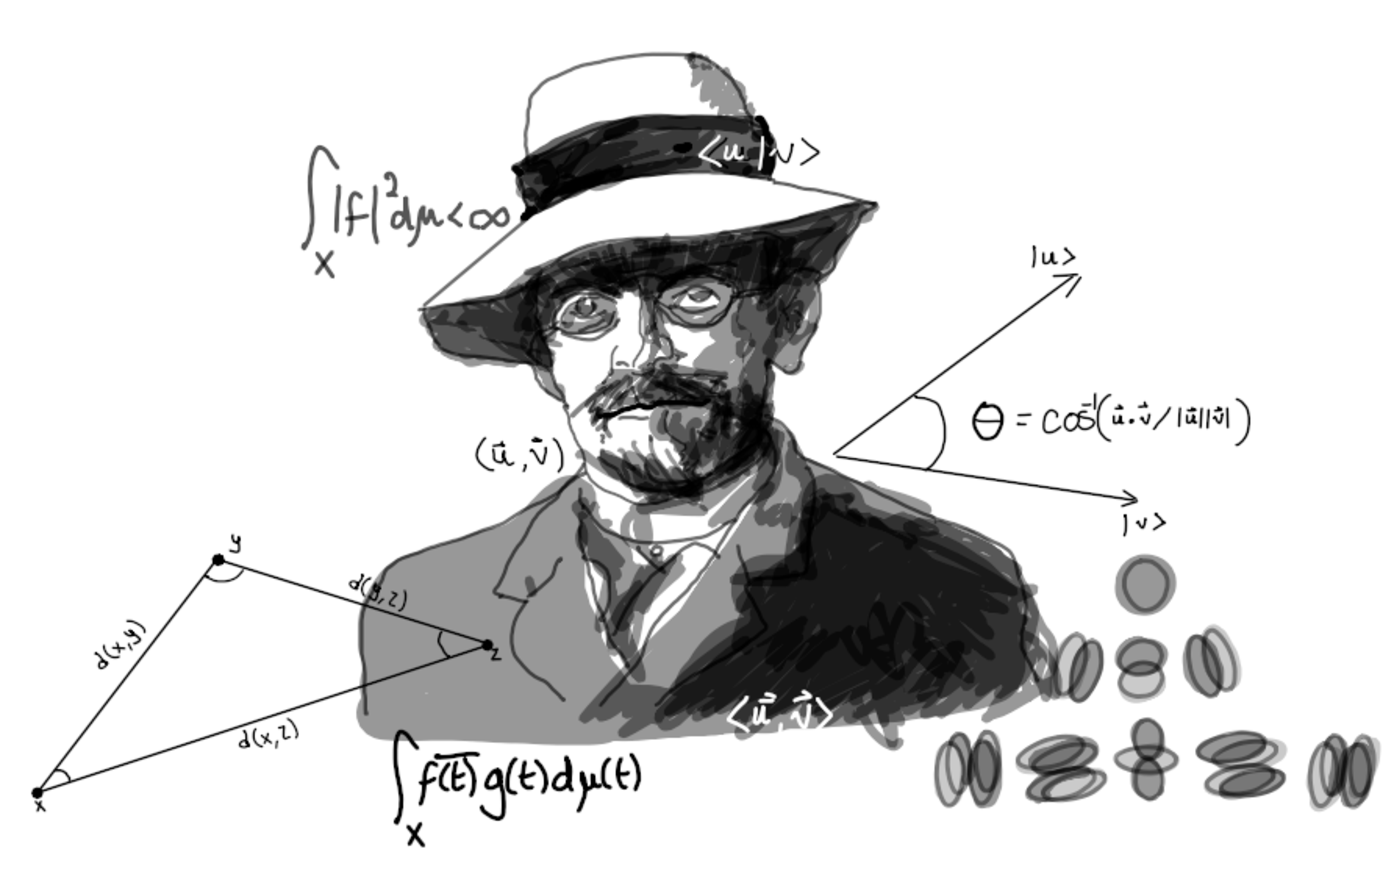
\includegraphics[width=0.6\textwidth]{hilbert.pdf}
    \\
    \tiny{Fig.1: Hilbert space stuff}
    \end{figure}
\end{frame}


\begin{frame}{Hamiltonians as Observables}
    \centering{
    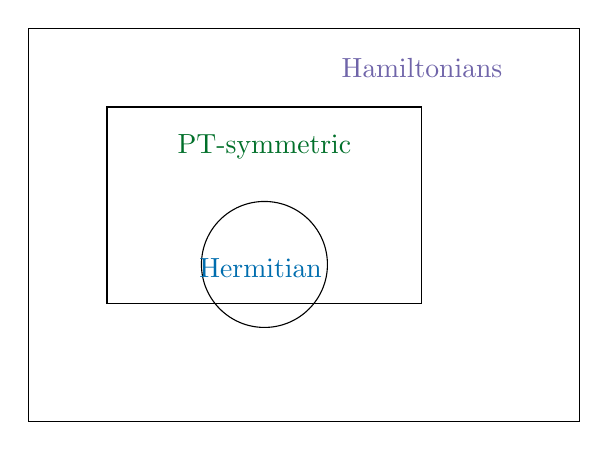
\begin{tikzpicture}
    \draw (-2,-1) rectangle(5,4) ++(-2,-0.5) node{\textcolor{myNewColorB}{Hamiltonians}};
    \draw (1,1) circle[x radius=0.8, y radius=0.8] ++(-0.05,-0.05) 
    node{\textcolor{myNewColorA}{Hermitian}};
    \pause
    \draw (-1,0.5) rectangle(3,3) ++(-2,-0.5) node{\textcolor{myNewColorC}{PT-symmetric}};
    \end{tikzpicture}}
    \\
    \hspace{1em}
    \begin{tiny}
        Fig.2: The set of all possible Hamiltonians.
    \end{tiny}
    \\
    \begin{enumerate}
        \item \textcolor{myNewColorA}{Observables are \textbf{self-adjoint} operators.}
        \item \textcolor{myNewColorC}{$\hat{H}$ has a real energy spectrum bounded below.}
        \item \textcolor{myNewColorC}{Unitarity.}
    \end{enumerate}
\end{frame}

\begin{frame}{PT - symmetry in short}
    \vspace{-1cm}
    \begin{align*}
        & \mathcal{P} \rightarrow \mathrm{spatial\:inversion},\\
        & \mathcal{T} \rightarrow \mathrm{time\:reversal\:(complex\: conjugation)}.
    \end{align*}\\
    \vspace{0.5cm}
    \begin{equation*}
    \hat{H} = \mathcal{PT}\:\hat{H}\:\mathcal{PT} = \hat{H}^{\mathcal{PT}} 
    \end{equation*}\\
    \vspace{0.5cm}
    \pause
    \begin{itemize}
    \item The $\mathcal{PT}$ inner product is determined dynamically in terms of the Hamiltonian.\\
    \pause
    \item $\mathcal{PT}$-symmetry can be \textbf{broken} or \textbf{unbroken}.
    \pause
    \item Interesting physical phenomena occurs in the broken symmetry region.
    \end{itemize}
\end{frame}


\section{Time evolution}
\begin{frame}{Time evolution}
\vspace{-1cm}
\hspace{-2em}
\vspace{2cm}
\begin{columns}[T]
    \begin{column}{0.3\textwidth}
    \vspace{-2cm}
    \begin{align*}
    &\Scale[2]{\vec{\psi_{i}} \rightarrow{} \vec{\psi_{f}}}
    \end{align*}
    \pause
    \hspace{6em}
    \Scale[2.2]{\hookrightarrow}
    \end{column}
    
    \begin{column}{0.8\textwidth}
    \vspace{-1.1cm}
    \Scale[3]{\vec{\psi_{f}} = \hat{U} \vec{\psi_{i}}}\\
    \pause
    \hspace{6.8em}
    \begin{huge}
    {$\downarrow$}\\
    \end{huge}
    \begin{itemize}
    \item \textcolor{myNewColorA}{Hermitian} quantum mechanics:\\
    \hspace{5em}
    $\hat{U} = e^{-i\hat{H}t / \hbar}$\\
    \hspace{5em}
    \pause
    \item \textcolor{myNewColorC}{PT} quantum mechanics:\\ 
    \hspace{5em}
    $\hat{U} = e^{-i\tilde{H}t / \hbar}$\\
    \hspace{5em}
    \pause
    \textcolor{myNewColorC}{\large{Unitary?}}
    \end{itemize}
    \end{column}
    \end{columns}
\end{frame}


\section{Brachistochrone problem}
\begin{frame}{The Classical Brachistochrone problem}
\vspace{0.5cm}
\begin{columns}
    \hspace{1.5em}
    \begin{column}{\textwidth}
    \multiinclude[format=pdf,start=1,graphics={width=0.5\textwidth}]
    {optim-gif/optimisation}
    \\
    \hspace{1em}
    \tiny{Fig.3:
    A particle travels from left to right in time t,\\
    \hspace{2.4em}
    Can we make this trip nearly instantaneous?}
    \end{column}
    
    \hspace{-15em}
    \begin{column}{0.5\textwidth}
        βράχιστος χρόνος\\
        brákhistos khrónos:\\
        ``shortest time"\\
    \vspace{1cm}
    \small{\textcolor{myNewColorC}{How fast can we evolve a state?}
    }
    \end{column}
    \end{columns}
\end{frame}


\begin{frame}{A simple quantum brachistochrone problem}
\begin{columns}
    \hspace{1.5em}
    \begin{column}{\textwidth}
    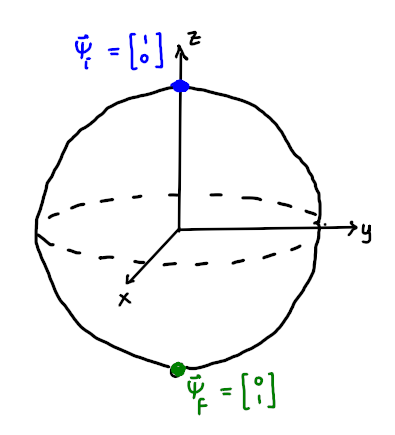
\includegraphics[width=0.35\textwidth]{bloch.png}\\
    \tiny{Fig.4: Bloch sphere with initial and final states}
    \end{column}
    \begin{column}{0.8\textwidth}
    \hspace{-18em}
    This space is spanned by $\vec{\psi_i}$ and $\vec{\psi_f}.$\\
    \vspace{0.4cm}
    \hspace{-18em}
    \pause
    What is the \textbf{fastest} time evolution possible,\\
    \hspace{-18em}
    that does not violate the\\
    \hspace{-18em}
     time-energy uncertainty principle.\\
    \vspace{0.4cm}
    \pause
    \hspace{-18em}
    The Hamiltonian must satisfy an\\ 
    \hspace{-18em}
    \textcolor{myNewColorD}{energy constraint} based on:\\
    \hspace{-15em}
    \textcolor{myNewColorD}{$\quad\omega  \equiv E_{\mathrm{max}} - E_{\mathrm{min}}$} $> 0$\\
    \vspace{0.7cm}
    \pause
    \hspace{-18em}
    \textcolor{myNewColorC}{Will a complex non-Hermitian Hamiltonian}\\
    \hspace{-18em}
    \textcolor{myNewColorC}{give time-optimal evolution?}
    \end{column}
    \end{columns}
\end{frame}


\begin{frame}{The Maths}
\vspace{-1cm}
\begin{equation*}
    \vec{\psi_{i}}  = \begin{pmatrix}
                        1 \\
                        0 \\                
    \end{pmatrix}\pause, 
    \quad
    \vec{\psi_{f}}  = \begin{pmatrix}
                        a \\
                        b \\                
    \end{pmatrix}
    = \begin{pmatrix}
                        0 \\
                        1 \\                
    \end{pmatrix}.
    \vspace{0.5cm}
    \end{equation*} \\
    \pause
    \begin{columns}
    \begin{column}{0.5\textwidth}
    \textcolor{myNewColorA}{Hermitian} case
    \hspace{-3em}
    \begin{scriptsize}
    \begin{equation*}
    \hat{H}  = \begin{pmatrix}
                s & r e^{-i\theta}  \\
                r e^{i \theta} & u  \\
                \end{pmatrix} , \{r, s, \theta, u\} \in \mathbb{R},
    \end{equation*}\\
    \pause
    \textcolor{myNewColorD}{Energy constraint}
    \hspace{-1.5em}
    \begin{equation*}
        \textcolor{myNewColorD}{\omega^2 = (s-u)^2 + 4r^2},
    \end{equation*}\\
    \pause
    Time evolution
    \hspace{-1.5em}
    \begin{equation*}
        \begin{pmatrix}
            a \\
            b \\                
            \end{pmatrix} = e^{\frac{-i(s+u)t}{2\hbar}}\begin{pmatrix}
            \cos(\frac{\omega t}{2\hbar}) - i \frac{s - u}{\omega} \sin(\frac{\omega t}{2\hbar})\\
            - i \frac{2r}{\omega} e^{i \theta} \sin(\frac{\omega t}{2\hbar}) \\
            \end{pmatrix}.
    \end{equation*}\\
    \vspace{0.7cm}
    \end{scriptsize}
    \end{column}

    \begin{column}{0.5\textwidth}
    \textcolor{myNewColorC}{PT-symmetric} case
    \begin{scriptsize}
    \begin{equation*}
    \Tilde{H}  = \begin{pmatrix}
                r e^{i\theta} & s  \\
                s & r e^{-i\theta}  \\
                \end{pmatrix}, \quad \{r, s, \theta\} \in \mathbb{R},
    \end{equation*}\\
    \pause
    \textcolor{myNewColorD}{Energy constraint}
    \hspace{-1.5em}
   \begin{equation*}
        \textcolor{myNewColorD}{\omega^2 = 4s^2 - 4r^2 \sin^2{\theta}} > 0,
    \end{equation*}\\
    \pause
    Time evolution
    \hspace{-1.5em}
    \begin{equation*}
        \begin{pmatrix}
                a \\
                b \\                
        \end{pmatrix} = \frac{e^{\frac{-itr \cos\theta}{\hbar}}}{\cos{\alpha}}
        \begin{pmatrix}
                \cos(\frac{\omega t}{2 \hbar} - \alpha)\\
                - i \sin(\frac{\omega t}{2\hbar})\\
        \end{pmatrix}.
    \end{equation*}\\
    \hspace{-1.5em}
    where $\sin(\alpha) = \frac{r}{s}\sin(\theta)$.

    \end{scriptsize}
    \end{column}
\end{columns}
\end{frame}


\begin{frame}{The Maths}
\begin{scriptsize}
\begin{equation*}
    \vec{\psi_{i}}  = \begin{pmatrix}
                        1 \\
                        0 \\                
    \end{pmatrix}, \quad
    \vec{\psi_{f}}  = \begin{pmatrix}
                        a \\
                        b \\                
    \end{pmatrix}
    = \begin{pmatrix}
                        0 \\
                        1 \\                
    \end{pmatrix}
    \end{equation*}\\
    \end{scriptsize}
    \vspace{0.3cm}

    \begin{columns}
    \begin{column}{0.5\textwidth}
    \textcolor{myNewColorA}{Hermitian} time evolution\\

    \begin{scriptsize}
    \begin{equation*}
        \begin{pmatrix}
            a \\
            b \\                
            \end{pmatrix} = e^{\frac{-i(s+u)t}{2\hbar}}\begin{pmatrix}
            \cos(\frac{\omega t}{2\hbar}) - i \frac{s - u}{\omega} \sin(\frac{\omega t}{2\hbar})\\
            - i \frac{2r}{\omega} e^{i \theta} \sin(\frac{\omega t}{2\hbar}) \\
            \end{pmatrix}.
    \end{equation*}
    \pause
    \begin{equation*}
    \Rightarrow |b|= \frac{2r}{\omega} \sin\left(\frac{\omega t}{2\hbar}\right),
    \end{equation*}
    \pause
    \begin{equation*}
    \Rightarrow t = \frac{2\hbar}{\omega} \arcsin\left(\frac{\omega |b|}{2r}\right),
    \end{equation*}
    \pause
    For all $r>0$ subject to \textcolor{myNewColorD}{$\omega^2 = (s-u)^2 + 4r^2$}\\
    for a fixed $\omega$.
    \begin{equation*}
    \therefore \tau = \frac{2\hbar}{\omega} \arcsin\left(|b|\right) = \frac{\pi \hbar}{\omega}
    \end{equation*}\\
    is the minimum \textit{passage time}.
    \end{scriptsize}
    \end{column}

    \pause
    \begin{column}{0.5\textwidth}
    \vspace{2cm}
    \textcolor{myNewColorC}{PT} time evolution\\
    \vspace{-1cm}
    \begin{scriptsize}
    \begin{equation*}
        \begin{pmatrix}
                a \\
                b \\                
        \end{pmatrix} = \frac{e^{\frac{-itr \cos\theta}{\hbar}}}{\cos{\alpha}}
        \begin{pmatrix}
                \cos(\frac{\omega t}{2 \hbar} - \alpha)\\
                - i \sin(\frac{\omega t}{2\hbar})\\
        \end{pmatrix}.
    \end{equation*}\\
    \pause
    \begin{equation*}
    \Rightarrow |a|= \frac{\cos{\frac{\omega t}{2 \hbar} -\alpha}}{\cos{\alpha}} \sin\left(\frac{\omega t}{2\hbar}\right),
    \end{equation*}
    \pause
    \begin{equation*}
    \Rightarrow t = \frac{\hbar}{\omega}(2 \alpha + \pi) ,
    \end{equation*}
    \pause
    Since $\omega$ is fixed,
    \textcolor{myNewColorD}{$\omega^2 = 4s^2 - 4r^2 \sin^{2}(\theta)$}\\
    $\quad\quad\quad\quad\:\:\:\quad \to \omega^2 = 4s^2\cos^2(\alpha)$\\
    \pause
    \vspace{0.5cm}
    Then $t \to 0$ when $\alpha \to -\frac{\pi}{2}$.\\
    but we also require $s, r >> 1$.\\
    \end{scriptsize}
    \end{column}
\end{columns}
\end{frame}


\begin{frame}{The geometry of the space}
\begin{columns}
    \hspace{1.5em}
    \begin{column}{\textwidth}
    $\mathcal{PT}$ inner products are defined depending on the Hamiltonian used.\\
    \pause
    \vspace{0.5cm}
    \begin{equation*}
        \vec{\psi_i} = \begin{pmatrix}
                1 \\
                0 \\                
        \end{pmatrix}, \quad
        \vec{\psi_f} = \begin{pmatrix}
                0 \\
                1 \\                
        \end{pmatrix}
        \end{equation*}
    \begin{enumerate}
        \item orthogonal $\to$ \textcolor{myNewColorA}{Hermitian} inner product\\
        \pause
        vector separation: $\delta = 2 \arccos{|\left< \psi_{f}| \psi_{i}\right>|} = \pi$\\
        \pause 
        \item not orthogonal $\to$ \textcolor{myNewColorC}{PT}  inner  product\\
        \pause
        vector separation: $\delta = \pi - 2|\alpha|$\\
        \pause 
        \vspace{0.5cm}
        We can choose $\alpha$ to create a ``wormhole" effect in Hilbert space.
        \end{enumerate}
    \end{column}
\end{columns}
\end{frame}

\section{Conclusion}
\begin{frame}{Conclusion}
\begin{enumerate}
    \item This paper demonstrates the theoretical differences in both $\mathcal{PT}$-symmetric and conventional Hermitian quantum mechanics.\\
    \item The ``wormhole" effect could be of importance in design and implementation of fast quantum computation and comunication algorithms.\\
    \item There could be quantum protection mechanisms limiting the applicability of Hilbert-space ``wormholes".
\end{enumerate}
\end{frame}

\begin{frame}{References} 
    \nocite{*}
    \bibliographystyle{unsrturl_mod}
    \bibliography{mybib.bib}
\end{frame}

\pause

% \section{Appendix}
\begin{frame}{This paper's abstract}
\begin{figure}
    \hspace{-4.8em}
    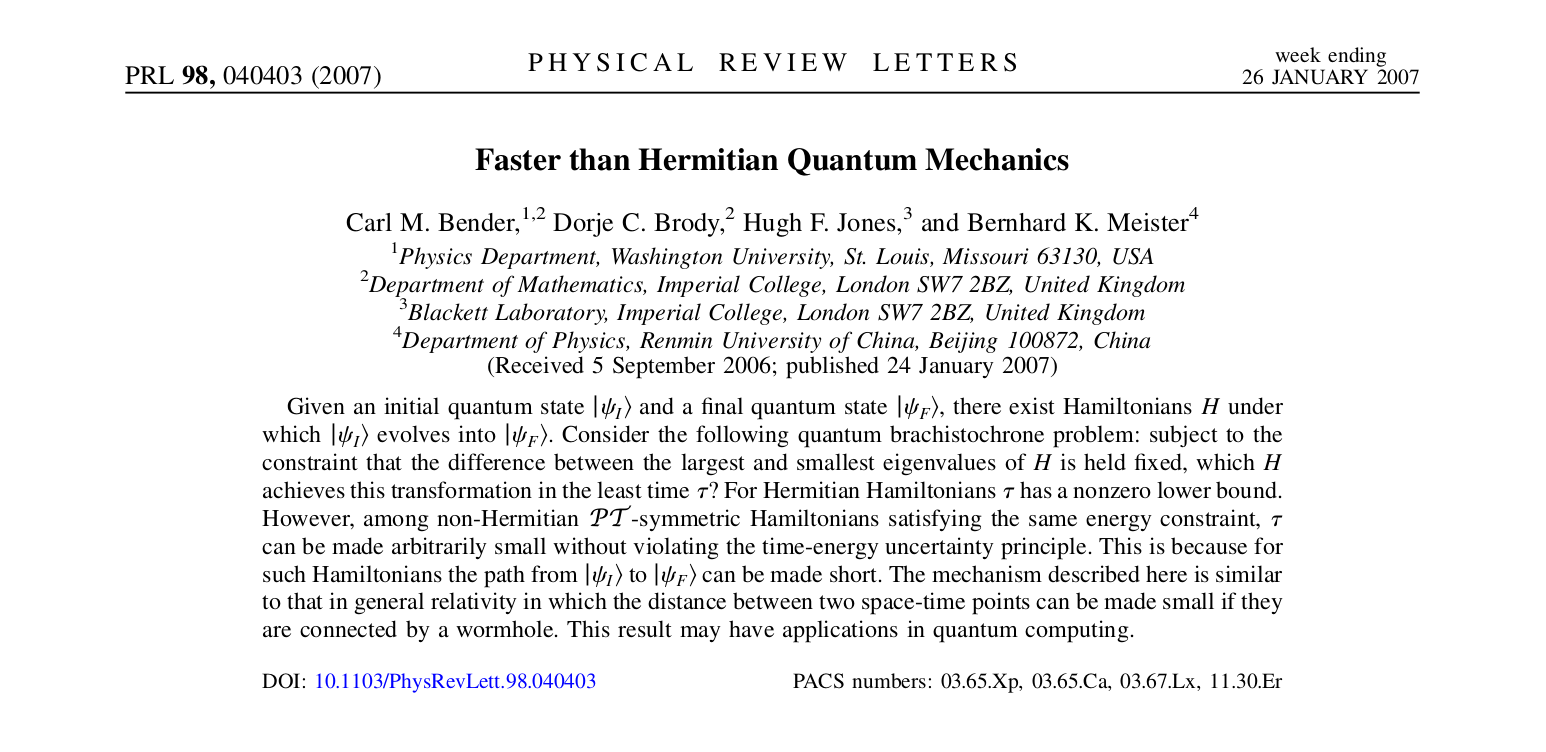
\includegraphics[width=1.13\textwidth]{paper.png}
    \\
    \tiny{}
    \end{figure}
\end{frame}

\begin{frame}{Broken PT-symmetry phenomena}
\begin{figure}
    \hspace{-4.5em}
    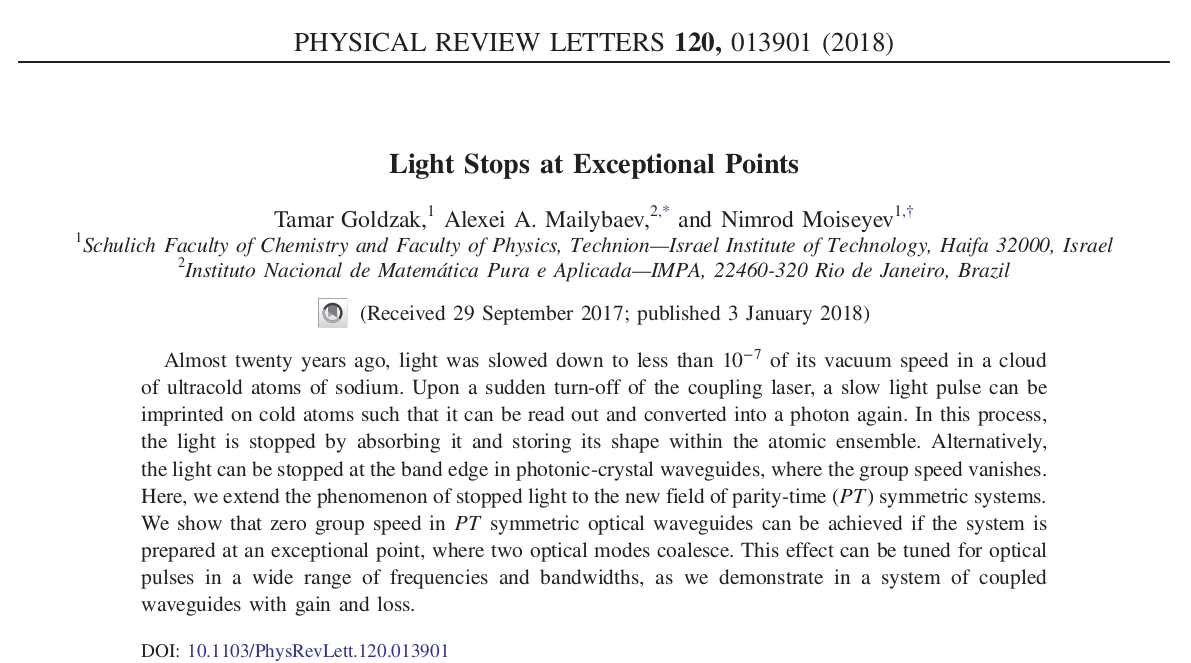
\includegraphics[width=\textwidth]{lightstops.png}
    \\
    \tiny{}
    \end{figure}
\end{frame}

\begin{frame}{Broken PT-symmetry phenomena}
\begin{figure}
    \hspace{-4.5em}
    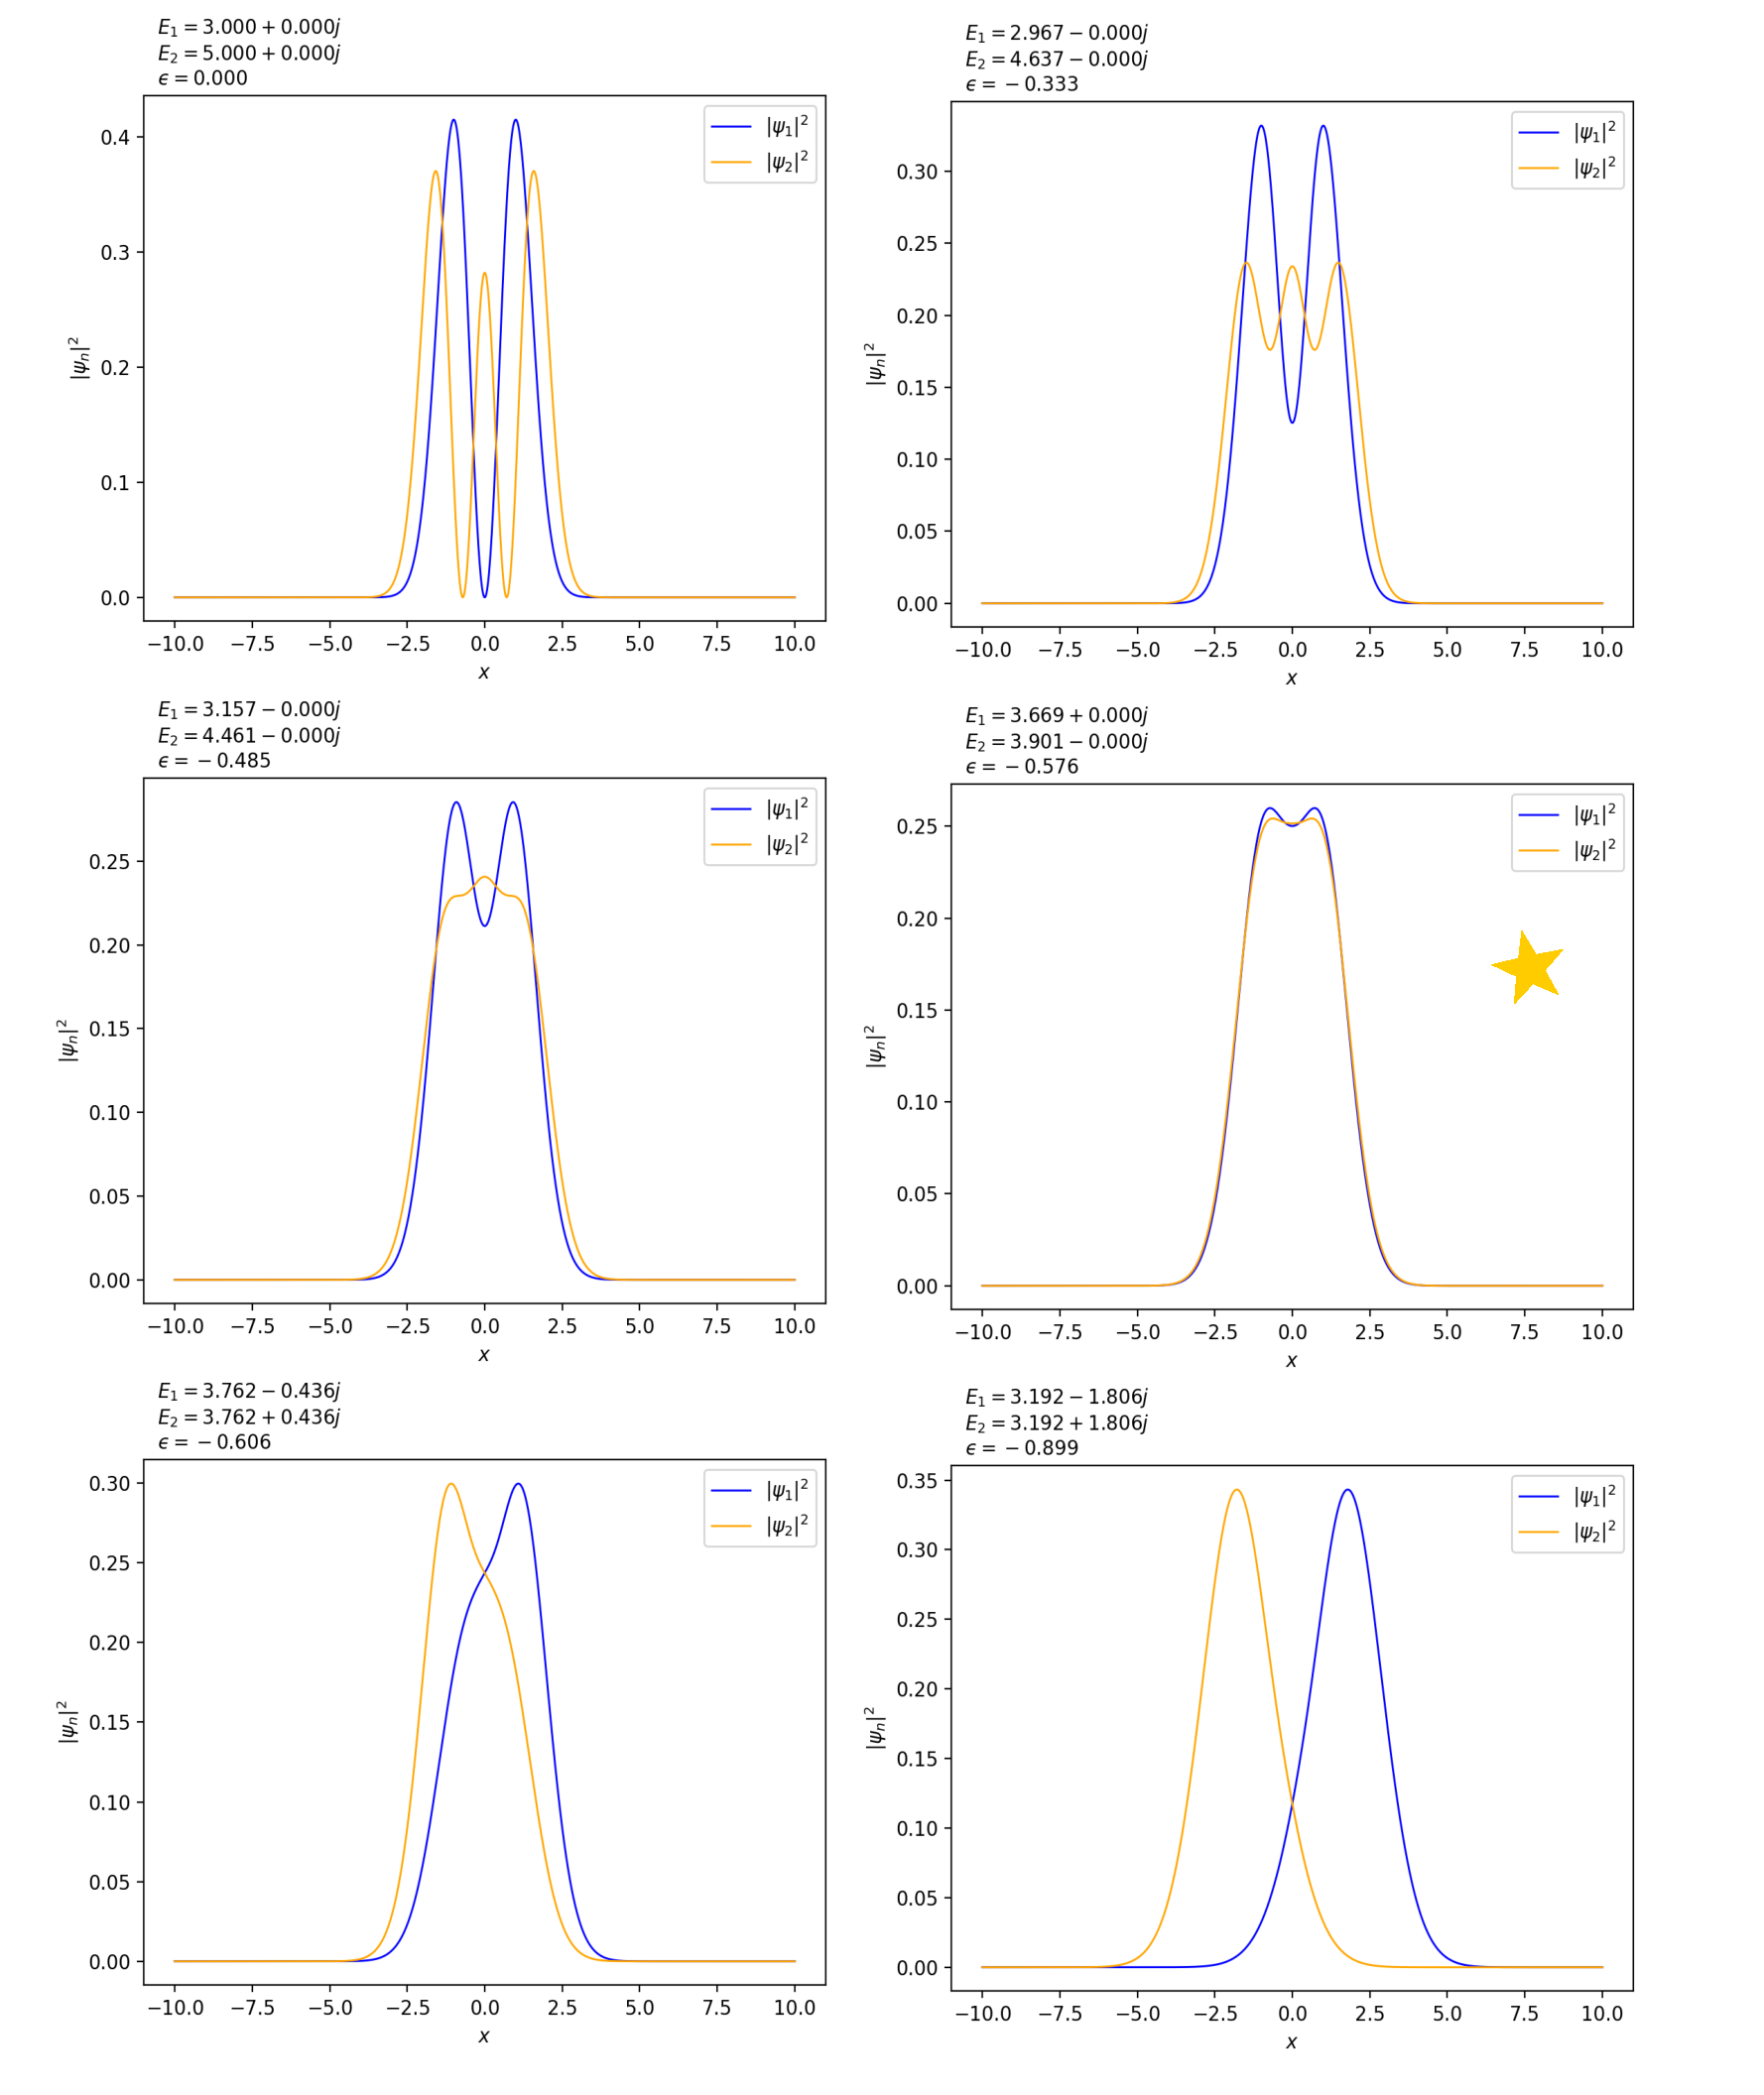
\includegraphics[width=0.5\textwidth]{amplitudes.pdf}
    \\
    \tiny{Fig 5. The probability density of the wave functions corresponding to the first and second excited states of the harmonic oscillator. States' probability densities are symmetric about zero. As the exceptional point parametric value is approached from the left, the probability densities begin to overlap in space. We can see the densities of the wave functions behave as mirror images of each other after we pass the exceptional point in the negative direction.}
    \end{figure}
\end{frame}

\begin{frame}{Constructing the PT inner product}
The $\mathcal{PT}$ inner product is \textbf{not positive definite}.\\
To patch up this problem, we use the $\mathcal{C}$ operator:\\
\begin{equation*}
\mathcal{C} \rightarrow \mathrm{charge\: conjugation}
    \end{equation*}\\
\begin{equation*}
\mathcal{C}^2 = 1,\quad [\mathcal{C}, \hat{H}] = 0,\quad [\mathcal{C},\mathcal{PT}] = 0.
    \end{equation*}\\
\vspace{0.5cm}
We construct $\mathcal{C}$ from the $\hat{H}$ eigenstates $\psi_n$.\\
\begin{equation*}
\mathcal{C} = \sum_{n} \psi_{n}(x) \psi_{n}(y)
    \end{equation*}\\
Inner product: 
\begin{equation*}(\mathcal{CPT} \psi_{n}(x)) \cdot \psi_{m}(y) = \mathcal{C} \psi^{*}_{n}(-x)) \cdot \psi_{m}(y)
\end{equation*}
\end{frame}

% \begin{frame}{Equivalent Hermitian and PT symmetic Hamiltonians}
% For any Hamiltonian with unbroken $\mathcal{PT}$-symmetry there exists an equivalent Hermitian Hamiltonian.
% \begin{enumerate}
%     \item
% \end{enumerate}
% \end{frame}

\end{document}





